\capitulo{3}{Conceptos teóricos}\label{conceptos teoricos}

Este proyecto se centra principalmente en investigación, por lo que tiene una importante carga teórica. En el apéndice del cuaderno de investigación se explica el uso de todas las técnicas que hemos empleado en los experimentos, especificando implementaciones concretas, parámetros utilizados y resultados obtenidos. Por otra parte, en este apartado se van a exponer los conceptos teóricos en los que se basan esas técnicas sin entrar en los detalles de implementación.  

Dado que el desarrollo de la investigación se ha basado en el proceso \textit{KDD} (explicado más detenidamente en el apartado de Técnicas y Herramientas), este apartado se estructurará en función de los pasos que incluye este proceso: 

\section{Obtención de datos}

Los datos se obtienen de un colchón con sensores de presión en forma de tubo integrados en su interior como representa la figura~\ref{fig:ngmatt}. Además, el colchón cuenta con un sensor de constantes vitales. Juntando los datos obtenidos por cada tipo de sensor disponemos de los siguientes atributos: 

\begin{itemize}
	\item \textbf{MAC\_NGMATT} y \textbf{UUID\_BSN}: identificador del colchón asociado a los tubos de presión e identificador del sensor de biométricas (constantes vitales) respectivamente. 
	\item \textbf{DateTime}: día y hora en la que fue tomada cada lectura de datos. 
	\item \textbf{P1, P2, P3, P4, P5, P6, P7, P8, P9, P10, P11, P12}: presiones, en mBar, captadas por los 12 tubos de presión integrados en el colchón. 
	\item \textbf{HR} (\textit{Heart rate}): frecuencia cardíaca medida en pulsaciones por minuto. 
	\item \textbf{RR} (\textit{Respiration rate}): frecuencia de respiración medida en respiraciones por minuto. 
	\item \textbf{SV} (\textit{Stroke volume}): volumen sistólico medido en mililitros. 
	\item \textbf{HRV} (\textit{Heart rate variability}): variabilidad de la frecuencia cardíaca medida en milisegundos. 
	\item \textbf{B2B} (\textit{Beat to beat}): tiempo entre pulsaciones medido en milisegundos. 
	\item \textbf{SS}: potencia de la señal relativa a la matriz de tubos de presión. Un valor superior a 400 se considera aceptable. 
	\item \textbf{STATUS}: estado de medición del sensor de constantes vitales. 0=\textit{low signal}, 1=\textit{ok signal}, 2=\textit{high signal}, 3=\textit{close to overload}, 4=\textit{close to max HR}. 
\end{itemize}

Por otra parte se nos proporcionaron unos rangos aproximados de horas en los que el paciente tuvo un ataque epiléptico, lo que nos permite etiquetar cada instancia de datos como <<crisis>> o <<no crisis>>.  

\begin{figure}[H]
	\centering
	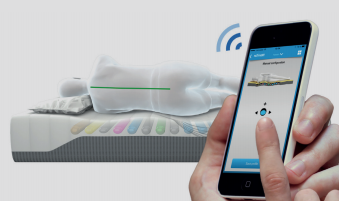
\includegraphics[width=0.8\textwidth]{../img/ngmatt.png}
	\caption{Imagen proporcional del colchón \textit{NGmatt2.0}.}
	\label{fig:ngmatt}
\end{figure}

\section{Limpieza de datos}

La limpieza de datos consiste en eliminar los datos inconsistentes o con ruido para evitar su interferencia en la extracción de conocimiento. 

\subsection{Eliminación de instancias por baja señal}

Dos de estos atributos, SS y STATUS, hacen referencia a la calidad de las instancias de los datos, uno haciendo referencia a la matriz de tubos de presión y otro al sensor de constantes vitales. Dado que la fase de limpieza de datos consiste en eliminar el ruido y las instancias incorrectas, es aquí donde eliminaremos todas las instancias cuyos datos no consideremos fiables en función de los valores de estos dos atributos. 

\subsection{Eliminación manual del ruido}

Una opción para eliminar el ruido de los datos es hacerlo de forma manual, inspeccionando los datos disponibles y modificando o eliminando aquellos que sean inconsistentes.  

\subsection{Eliminación del ruido mediante filtrado}

Otra forma de eliminar el ruido de una señal consiste en usar filtros. Un filtro es un sistema que se aplica a una señal (en nuestro caso la señal de presiones en el tiempo) y la transforma para conseguir un objetivo concreto, en este caso el suavizado de la señal para eliminar el ruido. Se han probado dos tipos de filtro distintos: 

\begin{itemize}
	\item \textbf{Filtro de Butterworth}~\cite{wiki:butterworth,scipybutter}: Diseñado para filtrado de señales eléctricas, trata de producir la respuesta más plana que sea posible hasta la frecuencia de corte (\textit{Wn}), dicho de otra forma, trata de mantener intactas las frecuencias por debajo de la frecuencia de corte mientras disminuye las frecuencias superiores con razón proporcional a \textit{N}, siendo \textit{N} el orden de filtrado:
	\begin{center}
		$|H| = \dfrac{1}{\sqrt{1+(W/Wn)^{2N}}}$
	\end{center}

	\begin{figure}[H]
		\centering
		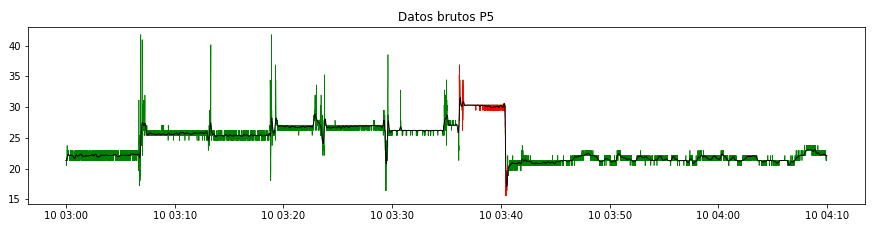
\includegraphics[width=1\textwidth]{../img/senalP5butter.png}
		\caption[Señal de presión (P5) filtrada con Butterworth.] {Ejemplo de señal de presión (P5) filtrada mediante un filtro de Butterworth con \textit{N}=3 y \textit{Wn}=0.05. En verde la señal original y en negro la señal filtrada.}
		\label{fig:senalP5butter}
	\end{figure}
	
	\item \textbf{Filtro de Savitzky–Golay}~\cite{wiki:savitzkygolay,scipysavgol}: Se basa en el cálculo de una regresión polinomial local para la que se debe especificar un tamaño de ventana (\textit{window\_lenght}) y el orden del polinomio utilizado en la regresión (\textit{polyorder}). 
	
	\begin{figure}[H]
		\centering
		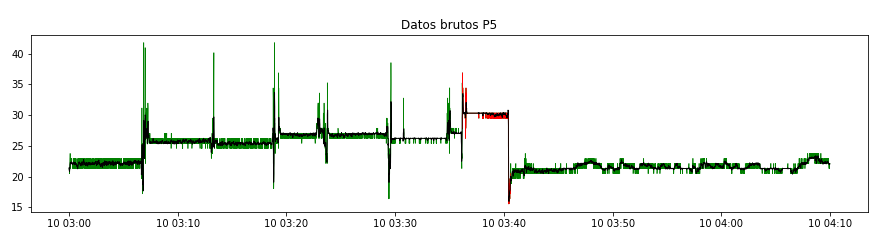
\includegraphics[width=1\textwidth]{../img/senalP5savgol.png}
		\caption[Señal de presión (P5) filtrada con Svatzky-Golay.]{Ejemplo de señal de presión (P5) filtrada mediante un filtro de Svatzky-Golay con \textit{window\_length}=15 y \textit{polyorder}=2. En verde la señal original y en negro la señal filtrada}
		\label{fig:senalP5savgol}
	\end{figure}
\end{itemize}

\subsection{Eliminación de atributos inconsistentes}

Al trabajar con datos reales, cabe la posibilidad de que algunos de los atributos contengan datos inconsistente, ya sea por que se produjeron errores (humanos o sistemáticos) durante la captación de los mismos o porque se corrompieron o perdieron durante su almacenamiento o su envío. Estos datos deberán ser eliminados para no interferir en la fase de minería de datos. Como se explicará en el apartado \ref{aspectos relevantes} (Aspectos Relevantes), en esta fase nos vimos obligados a eliminar los datos relativos a las constantes vitales. 

\section{Integración de datos}

Los datos disponibles corresponden con las instancias recogidas a lo largo de varios meses de una sola cama (un solo paciente). Estos datos nos han sido proporcionados en varios archivos de extensión .csv, por lo que la fase de integración ha consistido en recoger los datos en varios subconjuntos, uno por cada noche, considerando que una noche corresponde con el periodo de tiempo en el que el paciente estuvo acostado en la cama de forma ininterrumpida. 

\section{Selección de datos}

La selección de los datos consiste en desechar aquellos atributos o instancias que no resultan útiles para la extracción de conocimiento. A estas alturas del proceso, se siguen teniendo datos relativos a la identificación del colchón, a la hora en la que se tomó la instancia de dato y a las presiones. 

\subsection{Eliminación de identificadores}

Al contar con los datos de un único paciente, los atributos de identificación de la cama MAC\_NGMATT y UUID\_BSN no proporcionan ningún tipo de información útil para la extracción de conocimiento, por lo que ni siquiera son tenidos en cuenta en la fase de integración. 

\subsection{Eliminación de atributos de baja variabilidad}

Este proceso consiste en detectar aquellos atributos que varían menos de un umbral determinado durante el tiempo, y por lo tanto no proporcionarán información relevante. Como se explicará en el apartado \ref{aspectos relevantes} de Aspectos relevantes, este proceso nos llevó a desechar la mitad de los datos relativos a los tubos de presión. 

En este punto ya hemos seleccionado los atributos que serán considerados como \textbf{Datos en Bruto}: DateTime, P1, P2, P3, P4, P5 y P6.

\subsection{Selección de atributos para el entrenamiento}

Tras la fase de transformación de datos, la cual se abordará a continuación, se contará con una gran cantidad atributos calculados a partir de los datos en bruto. En la mayoría de los casos, resulta más eficiente entrenar el modelo de clasificación solo con un subconjunto de ellos que proporcione la mayor imformación, y por ello es necesario plantear estrategias para seleccionar el mejor subconjunto. En este proyecto se han planteado dos estrategias distintas: 

\begin{itemize}
	\item Escoger los atributos mejor situados en un ranking elaborado en función del rendimiento del clasificador en base a una métrica de evaluación concreta (estos conceptos se explican en fases posteriores). 
	\item Emplear un algoritmo genético para encontrar el mejor subconjunto de atributos. 
\end{itemize}

\subsubsection{Algoritmo genético}

Un algoritmo genético~\cite{koza92} es un método iterativo de búsqueda y optimización inspirado en la evolución biológica y el mecanismo de selección natural. En el contexto de un algoritmo genético una posible solución del problema se denomina <<individuo>>, y en cada iteración el algoritmo trabajará con un conjunto de individuos llamado <<población>> o <<generación>>. Los individuos tienen dos tipos de representación: 
\begin{itemize}
	\item \textbf{El genotipo:} es la representación del individuo que se empleará en las operaciones de cruce y mutación. 
	\item \textbf{El fenotipo:} es la representación del individuo que se empleará en la operación de evaluación. 
\end{itemize}

En cada iteración (o generación) se llevarán a cabo 4 operaciones: 
\begin{enumerate}
	\item \textbf{Selección} de los mejores individuos de la generación en base a una función de evaluación, que en nuestro caso se basará en el rendimiento de un clasificador entrenado con los atributos indicados por el individuo. 
	\item \textbf{Cruce} de algunos de los mejores individuos generando otros nuevos mediante la combinación de sus genotipos. 
	\item\textbf{Mutación} de algunos de los mejores individuos generando otros nuevos mediante la modificación de una pequeña parte de sus genotipos.
	\item \textbf{Reemplazo} de los individuos de la anterior generación por los nuevos individuos generados.  
\end{enumerate}

Cada uno de estos pasos puede emplear distintos mecanismos o implementaciones en función del genotipo de los individuos, el tipo de problema y otras consideraciones a tener en cuenta. 

\section{Transformación de datos}

\subsection{Técnicas de reducción de la dimensionalidad}

El primer tipo de transformación de datos que se utilizó fueron las técnicas de reducción de dimensionalidad~\cite{fodor2002dimreduction}. Estas técnicas consisten en proyectar datos en un plano, reduciendo su dimensión (número de atributos de cada instancia, en nuestro caso seis) a dos. Este tipo de enfoques se basan en la hipótesis de que la dimensionalidad de los conjuntos de datos es artificialmente alta, y que se puede mantener la misma información con una representación de los mismos con una dimensionalidad menor. 

\begin{figure}[H]
	\centering
	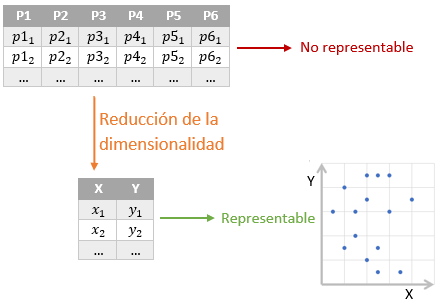
\includegraphics[width=0.7\textwidth]{../img/reducdim.png}
	\caption{Abstracción de la reducción de la dimensionalidad de los datos.}
	\label{fig:reducdim}
\end{figure}


Con esto, el objetivo que se persiguió fue comprobar si las instancias de <<crisis>> eran fácilmente separables de las instancias de <<no crisis>> en una representación bidimensional de los datos. Existen varios tipos de técnicas, cada una basada en unos criterios concretos para realizar la proyección, y se pueden clasificar principalmente en transformaciones lineales y transformaciones no lineales.  

\subsubsection{Transformaciones lineales}

Este tipo de transformaciones suponen que los datos observados son combinación lineal de una cierta base, y en ellas se engloba el \textbf{Análisis de Componentes Principales} (\textit{PCA})~\cite{pca}. 

\textit{PCA} es una de las técnicas más utilizadas y consiste en escoger el nuevo sistema de coordenadas (o base) de forma que se maximice la varianza entre las instancias. Cabe destacar que, para el nuevo sistema de coordenadas, se puede escoger cualquier dimensionalidad menor o igual a la del conjunto original de datos. Sin embargo, a mayor dimensionalidad, mayor coste de computación, y no es posible representar en papel proyecciones de más de 2 dimensiones, por lo que solo se ha probado esta última. 

\begin{figure}[H]
	\centering
	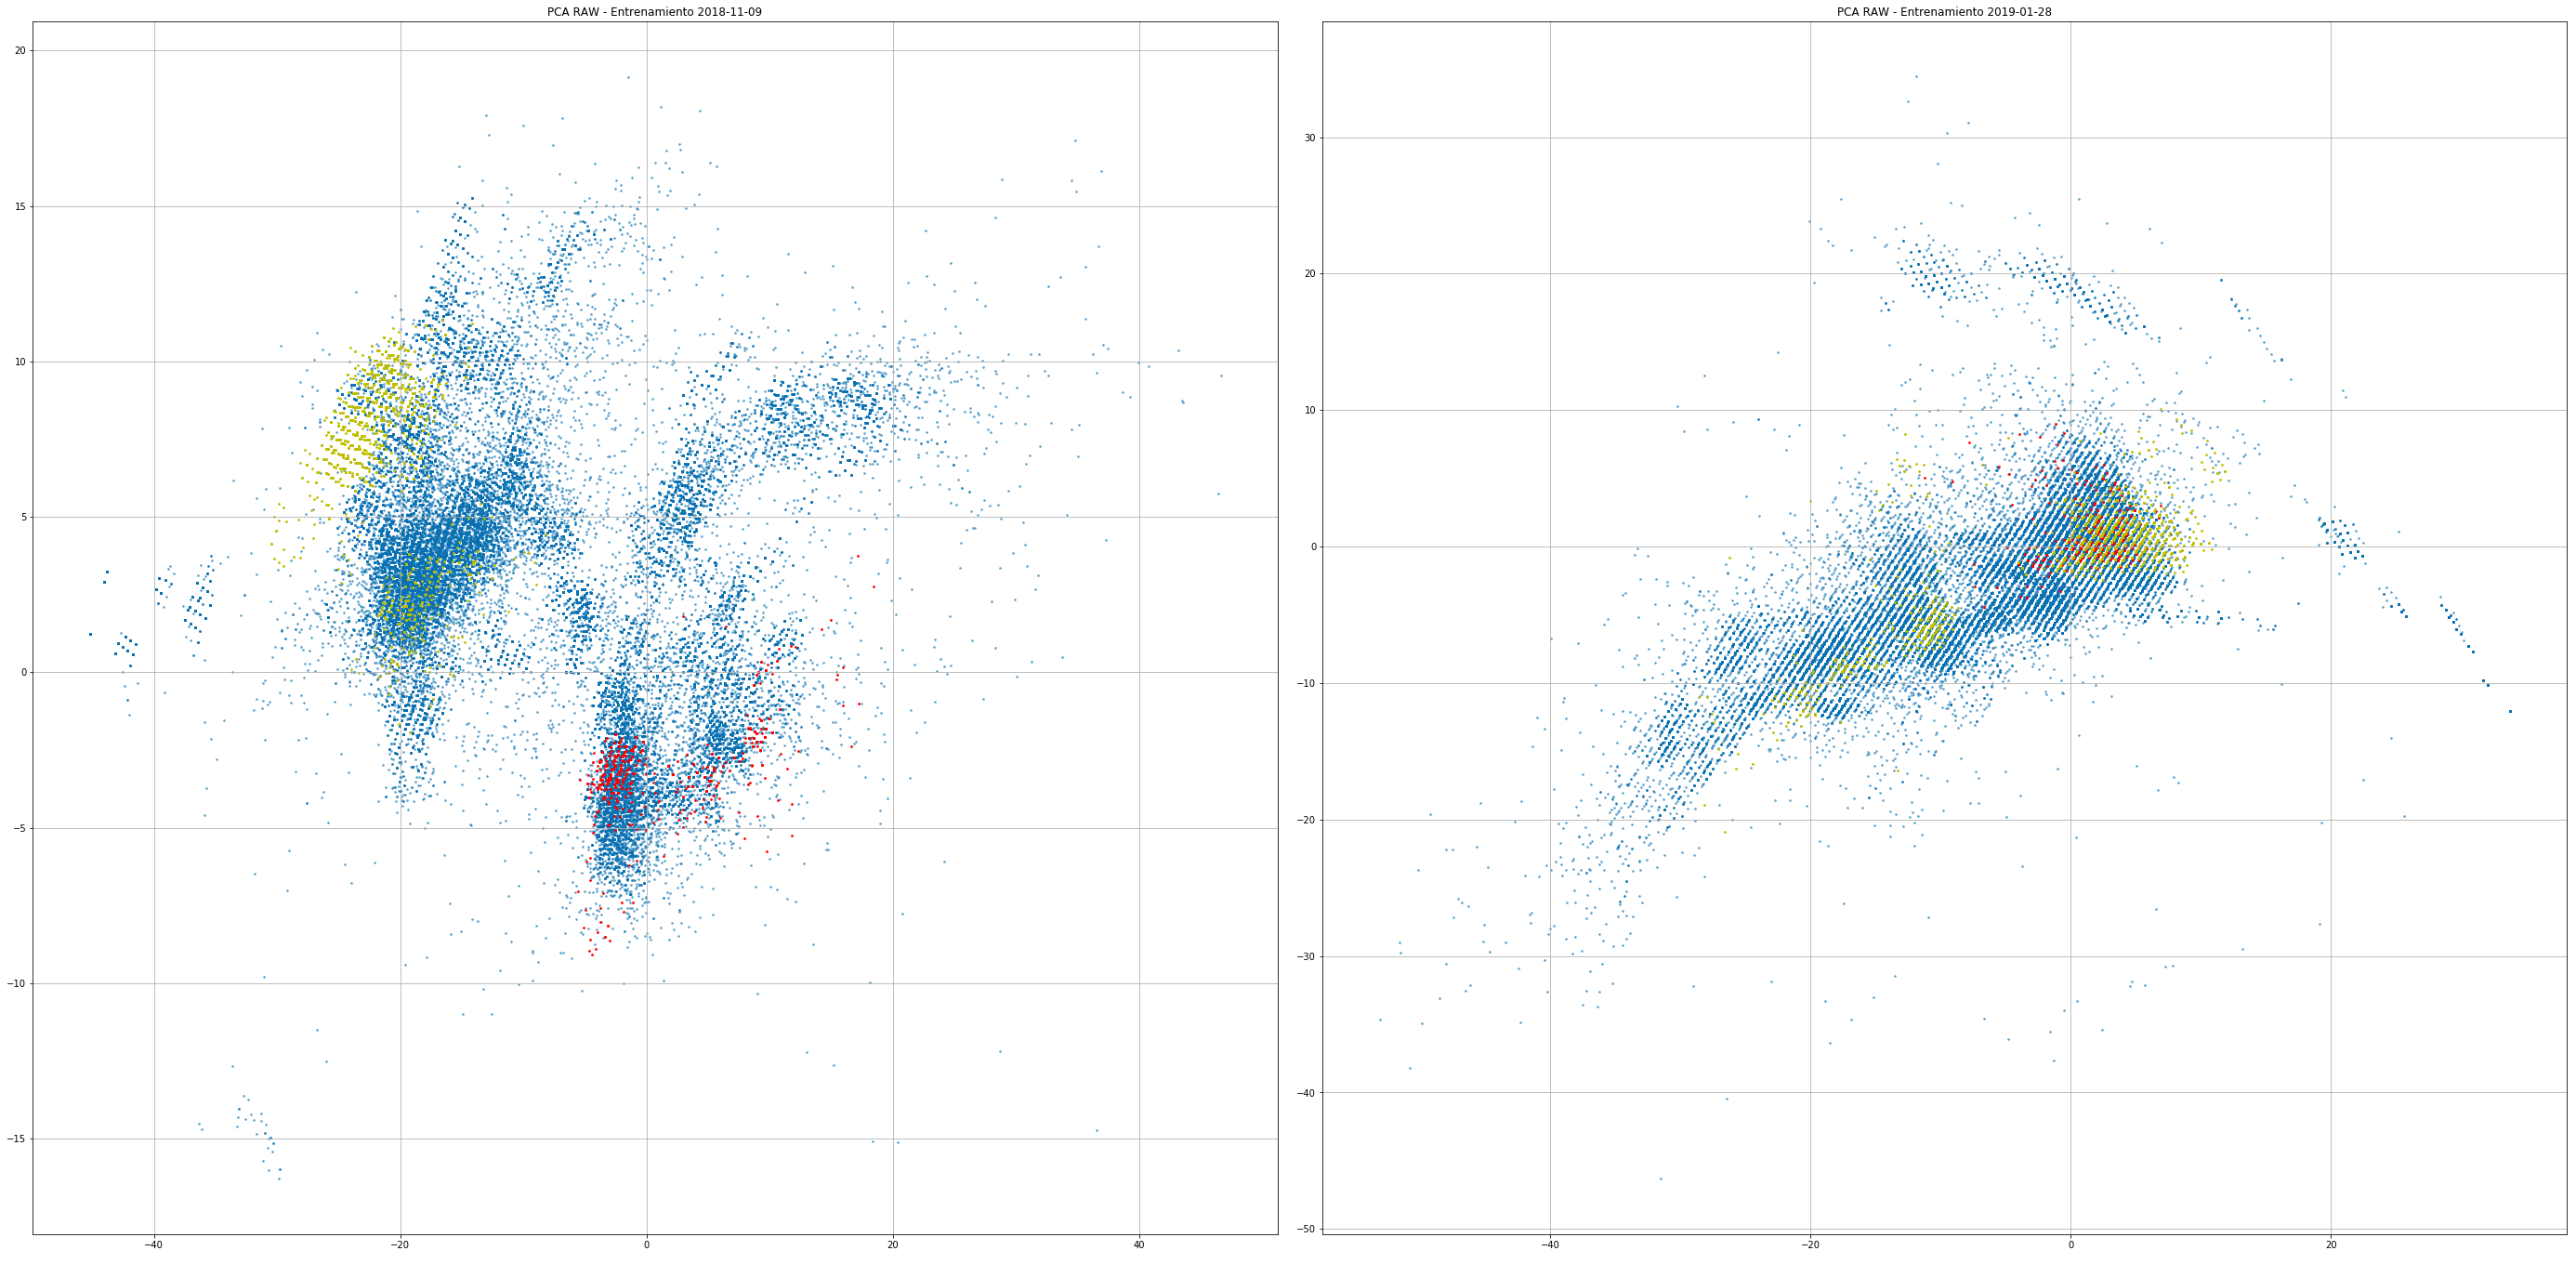
\includegraphics[width=1\textwidth]{../img/pca.png}
	\caption[Ejemplo de \textit{PCA}.] {\textit{PCA} aplicado a la noche de la crisis 1 (izquierda) y a la noche de la crisis 2 (derecha).}
	\label{fig:pca}
\end{figure}

En la figura~\ref{fig:pca}, los puntos rojos corresponden con instancias de <<crisis>> y los azules con instancias de <<no crisis>>. Como se puede ver no existe separación entre ellas. Los puntos amarillos corresponden con instancias de la otra crisis, y se puede ver que tampoco comparten espacio. 

\subsubsection{Transformaciones no lineales}

Las transformaciones no lineales~\cite{manifold}, no asumen que los datos sean una combinación lineal de una base. Existen varias técnicas de este tipo y en nuestro caso se han probado con éxito las siguientes: 

\begin{itemize}
	\item \textbf{\textit{Isomap}~\cite{isomap}:} Trata de reducir la dimensionalidad manteniendo las distancias geodésicas entre todas las instancias.
	\item \textbf{\textit{Locally Linear Embedding} (\textit{LLE})~\cite{lle}:} Reduce la dimensionalidad preservando las distancias dentro de los <<vecindarios>> locales. Se puede considerar como un conjunto de \textit{PCA}s locales que se comparan globalmente para encontrar la mejor reducción no lineal. 
	\item \textbf{\textit{Multi-Dimensional Scaling} (\textit{MDS}):~\cite{mds}} Es una técnica bastante utilizada en marketing y ciencias sociales que se basa en la similitud o disimilitud de los datos. Busca reducir la dimensionalidad tratando las distancias como valores proporcionales a la disimilitud de las instancias (lo que se parecen entre ellas).   
\end{itemize}

\begin{figure}
	\centering
	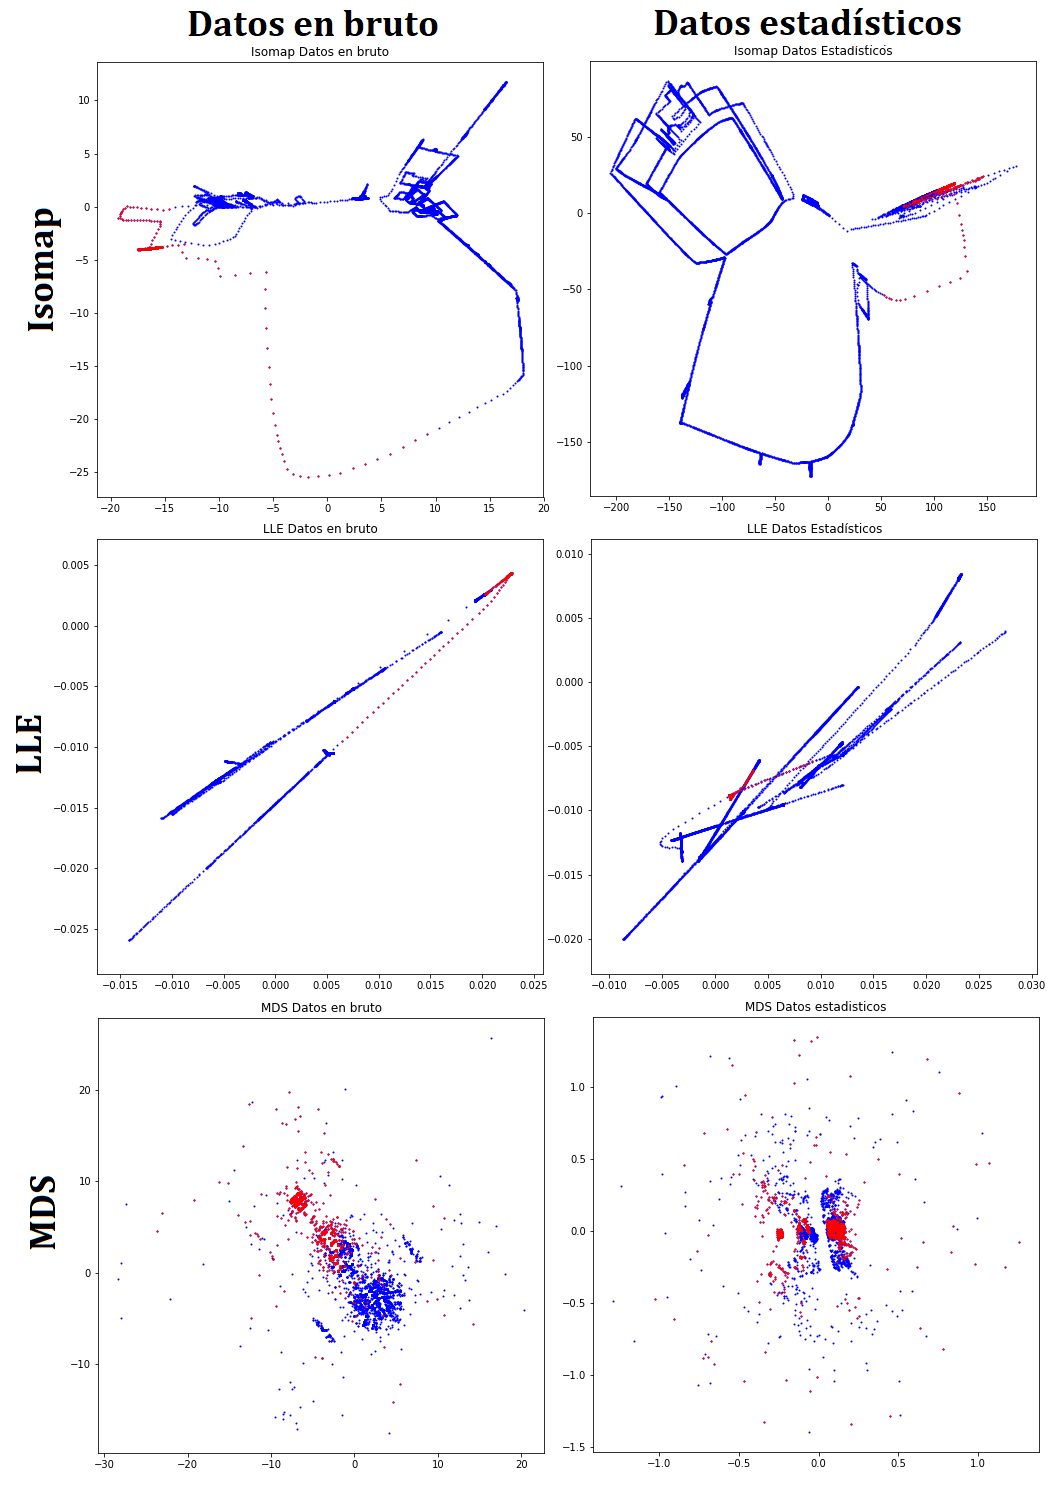
\includegraphics[width=1\textwidth]{../img/manifolds.png}
	\caption{Comparativa de las técnicas de transformación no lineal con los datos en bruto y usando estadísticos.}
	\label{fig:manifolds}
\end{figure}

Como se aprecia en la figura~\ref{fig:manifolds} con algunas de estas técnicas se consigue un grado algo mayor de separación, pero las instancias siguen sin ser fácilmente separables. En este caso, y como se puede observar, hemos aplicado las técnicas no solo a los datos en bruto, sino también a los datos estadísticos, lo que nos lleva al siguiente tipo de transformación. 

\subsection{Cálculo de estadísticas móviles}

En problemas donde los datos tienen una componente temporal las técnicas de minería de datos se pueden aplicar directamente a los datos en bruto, pero en ocasiones ofrecen un mejor rendimiento aplicadas a datos estadísticos calculados a partir de estos. Para calcular estadísticas móviles se debe definir el tamaño de la ventana (\textit{N}), de forma que para cada ventana se calculará un valor estadístico a partir de los datos contenidos en ella. Se han usado tres estadísticas simples: 

\begin{minipage}{\linewidth}
\begin{itemize}
	\item \textbf{Media móvil:} Es el valor promedio de los valores contenidos en la ventana. 
	\begin{center}
		$ \overline{x}=\frac{1}{N}\sum_{i=1}^{N}x_{i}$
	\end{center}
	\item \textbf{Desviación típica móvil:} Es una medida de la dispersión de los valores contenidos en la ventana. 
	\begin{center}
		$ \sigma=\sqrt{\frac{1}{N-1}\sum_{i=1}^{N}(x_{i}-\overline{x})^2}$
	\end{center}
	\item \textbf{Rango móvil:} Es la diferencia entre el valor máximo y el valor mínimo de los contenidos en la ventana. 
\end{itemize}
\end{minipage}

\subsection{Cálculo de características de series temporales}

Además de las descritas en el apartado anterior, se pueden calcular multitud de estadísticas más complejas, como es el caso de las características de series temporales. 

Una serie temporal~\cite{wiki:serietemporal} no es más que una secuencia de instancias medidas en determinado momento de tiempo y ordenadas cronológicamente, por lo que nuestro conjunto de datos corresponde con la definición de serie temporal. Las series temporales se suelen usar para estudiar la relación causal entre diversas variables que cambian en el tiempo y pueden influirse entre sí. Para este cometido existen una serie de técnicas específicas basadas en cálculos estadísticos más complejos. 

\section{Minería de datos}

En esta fase se ha tratado de generar un modelo capaz de encontrar los patrones que definen una crisis epiléptica. Para ello el modelo debe ser capaz de aprender a partir de los datos y, en función de como lo haga, se puede hablar de dos tipos básicos de aprendizaje: supervisado y no supervisado. 

\begin{itemize}
	\item Un modelo de \textbf{aprendizaje supervisado} se entrena con un conjunto de datos etiquetado, es decir, que cada instancia de dato de entrenamiento tiene asociado un valor categórico que ofrece información sobre a qué clase pertenece (para un problema de clasificación) o un valor numérico (para un problema de regresión). Este es un problema de clasificación y las dos clases posibles son <<crisis>> o <<no crisis>>. Tras el entrenamiento, el modelo deberá ser capaz de etiquetar nuevas instancias de dato distintas a las que se han usado en el entrenamiento como instancias de <<crisis>> o <<no crisis>> basándose en lo aprendido. En definitiva, el ciclo de vida de un clasificador supervisado tiene dos fases: 
	\begin{enumerate}
		\item \textbf{Entrenamiento:} El modelo aprende a partir de un conjunto de datos etiquetado. 
		\item \textbf{Predicción:} El modelo predice la clase de un dato no etiquetado, es decir, cuya clase real se desconoce. 
	\end{enumerate}
	
	\item En el \textbf{aprendizaje no supervisado} el modelo no tiene conocimiento sobre a qué clase pertenece cada instancia. Con este tipo de aprendizaje se pueden, por ejemplo, agrupar los datos en subconjuntos en función de sus características. Las técnicas de reducción de la dimensionalidad podrían ser consideradas técnicas de aprendizaje no supervisado, ya que elaboran la proyección sin conocer la clase de cada instancia, pero podrían darnos información sobre la existencia de dos clases si en las proyecciones bidimensionales existiera una clara separación entre dos grupos (\textit{clusters}) de instancias. 
\end{itemize}

Por otra parte, dentro de los modelos de clasificación podemos distinguir entre clasificadores simples o \textit{ensembles}.

\begin{itemize}
	\item Los \textbf{clasificadores simples} emplean un solo modelo que será el encargado de predecir la clase de las nuevas instancias. 
	\item Los \textbf{\textit{ensembles}}~\cite{kuncheva2004combining} son conjuntos de clasificadores simples cuyas predicciones se combinan para obtener una predicción final. La idea es construir varios modelos que no necesariamente predigan la misma clase para la misma instancia, y será la combinación de estas predicciones, por ejemplo, mediante votación, la que determinará la clase que predice el \textit{ensemble}. Para que este sistema de clasificación tenga sentido los modelos que forman el \textit{ensemble} deben ser algo distintos entre sí, de lo contrario no ofrecerían ninguna ventaja, y esa diferencia puede radicar en varios mecanismos, por ejemplo: 
	\begin{itemize}
		\item \textbf{\textit{Ensembles} heterogéneos:} El \textit{ensemble} se compone de modelos obtenidos con distintos métodos. 
		\item \textbf{\textit{Ensembles} homogéneos:} Cada modelo se entrena con el mismo algoritmo. La diferencia entre modelos puede radicar en que: 
		\begin{itemize}
			\item El proceso de construcción del modelo no es determinista, por lo que al entrenar varias instancias de ese modelo no se generan clasificadores exactamente iguales. 
			\item Cada modelo se entrena con un conjunto de datos diferente.
			\item Cada modelo se entrena con un subconjunto de atributos diferente para el conjunto de datos. 
		\end{itemize}
	\end{itemize}
\end{itemize} 

\begin{figure}
	\centering
	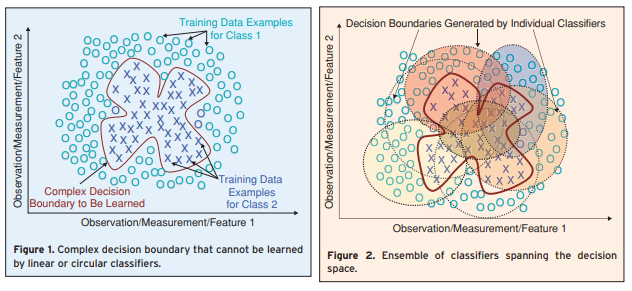
\includegraphics[width=1\textwidth]{../img/ensembles.png}
	\caption[Uso de \textit{ensembles} para problemas de clasificación complejos.]{Uso de \textit{ensembles} para problemas de clasificación complejos~\cite{polikar2006ensemble}.}
	\label{fig:ensemble}
\end{figure}

Teniendo en cuenta estas distinciones a continuación se exponen los modelos de clasificación que se han probado en este proyecto.

\subsection{Random Forest}

El clasificador \textit{Random Forest} es un \textit{ensemble} que emplea  árboles de decisión, y se trata de uno de los más sencillos y utilizados. Para construir cada árbol emplea la técnica de \textit{Bagging}, que consiste en entrenar cada modelo con un conjunto de datos del mismo tamaño que el original pero generado mediante muestreo uniforme con reemplazo (los datos pueden aparecer varias veces en el mismo conjunto). Mediante este mecanismo se reduce la varianza y se evita el sobreajuste. 

Además, durante la construcción de los árboles que componen el \textit{ensemble}, en cada nodo de decisión se tendrá en cuenta únicamente un subconjunto aleatorio de atributos del conjunto de datos.

Dado que todos los modelos del \textit{ensemble} son independientes los unos de los otros, tienen la misma importancia, por lo que su voto tendrá el mismo peso a la hora de calcular la predicción final. 


\subsection{AdaBoost.M1}

Se trata de un \textit{ensemble} para clasificación multi-clase que emplea aprendizaje supervisado. Emplea el método de \textit{Boosting}, que a diferencia de \textit{Bagging} es iterativo, y genera cada modelo del \textit{ensemble} influenciado por el rendimiento del anterior. En este caso se busca que cada modelo dé más importancia a las instancias que son mal clasificadas por el modelo anterior. A diferencia de \textit{Bagging} este mecanismo puede producir sobreajuste, sobre todo si el conjunto de datos tiene demasiado ruido. 

Debido a la forma en la que se construyen los modelos simples que lo componen, a la hora de calcular la predicción final para una nueva instancia el voto de cada modelo tendrá un peso distinto en función de su precisión.  

\begin{figure}[H]
	\centering
	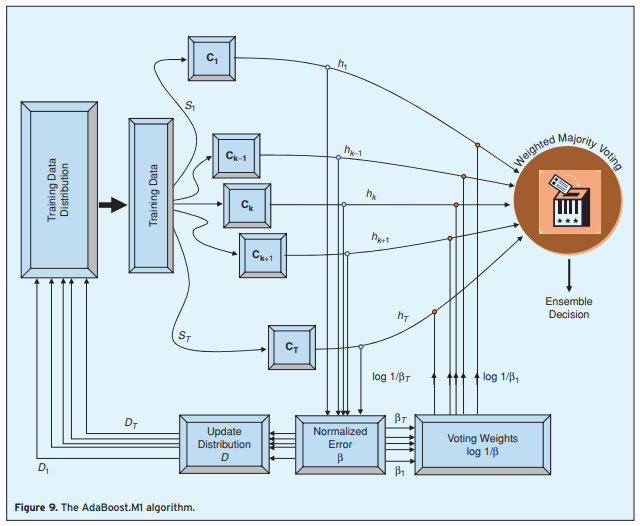
\includegraphics[width=0.8\textwidth]{../img/adaboostm1.png}
	\caption[Funcionamiento del algoritmo AdaBoost.M1.]{Funcionamiento del algoritmo AdaBoost.M1~\cite{polikar2006ensemble}.}
	\label{fig:adaboostm1}
\end{figure}

\subsection{Rotation Forest}

\textit{Rotation Forest}~\cite{rodriguez2006rotation} es también un \textit{ensemble} para clasificación que emplea aprendizaje supervisado mediante árboles de decisión. No se basa en un algoritmo iterativo como \textit{Boosting}, por lo que los clasificadores simples pueden ser generados de forma paralela. Se trata de un método algo más complejo que los anteriores, basado en la aplicación del ya mencionado \textit{PCA} a subconjuntos, preferiblemente disjuntos, de atributos. Para la obtención de las proyecciones se usan subconjuntos distintos de los datos, pero cada árbol se entrena con todas las instancias de entrenamiento. 

\subsection{One-Class}

La detección de anomalías One-Class consiste en entrenar el modelo con instancias de una sola clase de forma que a la hora evaluar nuevas instancias, devolverá información sobre si cada una pertenece o no a la clase. Esto lo realiza basándose, de alguna forma, en su similitud con las instancias usadas en el entrenamiento. 

Por ejemplo, si entrenamos el clasificador solo con instancias etiquetadas como <<no crisis>> y utilizamos datos de ambas clases para la predicción, esta puede devolver dos valores: 

\begin{itemize}
	\item La nueva instancia corresponde con la clase, por lo que se predice <<no crisis>>. 
	\item La nueva instancia no corresponde con la clase, por lo que se predice <<crisis>>. 
\end{itemize}

Durante el entrenamiento no se indica explícitamente a qué clase pertenece cada instancia, pero dado que todas las instancias de entrenamiento pertenecen a la misma, sí se le está proporcionando cierta información sobre la clase a la que pertenecen, y por lo tanto puede ser considerado como un algoritmo de aprendizaje supervisado. 

\section{Evaluación de patrones}

En el contexto de este trabajo, la utilidad de los patrones encontrados corresponderá con la precisión del clasificador en sus predicciones. Dado que al clasificar instancias nuevas no conocemos a priori la clase a la que pertenecen, no podemos saber si la clasificación ha sido correcta, por lo que para calcular la precisión de un clasificador se debe usar una partición de entrenamiento y test del conjunto original de datos disponibles: 

\begin{minipage}{\linewidth}
\begin{itemize}
	\item La \textbf{partición de entrenamiento} contiene la mayoría de los datos (por ejemplo, el 75\%), los cuales serán usados para entrenar el clasificador. 
	\item El resto corresponden con la \textbf{partición de test}, que serán usados para comparar su clase real (su etiqueta) con la clase predicha por el clasificador entrenado.
\end{itemize} 
\end{minipage} 

La precisión corresponde con el porcentaje de acierto del clasificador para la partición de entrenamiento, pero en ocasiones, conviene usar métricas más complejas para medir el rendimiento de un clasificador. En este trabajo se ha trabajado con dos métricas distintas: el área bajo la curva ROC y la precisión media, pero antes de explicarlos es necesario presentar algunos conceptos básicos.  

En un problema de clasificación binaria como este, si consideramos una instancia de <<crisis>> como un positivo (P) y una instancia de <<no crisis>> como un negativo (N) podemos definir los siguientes valores: 

\begin{itemize}
	\item Verdaderos positivos (TP): número de instancias de <<crisis>> que son clasificadas como <<crisis>>. 
	\item Falsos positivos (FP): número de instancias de <<no crisis>> que son clasificadas como <<crisis>>. 
	\item Verdaderos negativos (TN): número de instancias de <<no crisis>> que son clasificadas como <<no crisis>>. 
	\item Falsos negativos (FN): número de instancias de <<crisis>> que son clasificadas como <<no crisis>>.  
\end{itemize}

Estos valores se suelen visualizar en forma de matriz de confusión, la cual tiene la estructura de la figura~\ref{fig:matrizconfusion}.

\begin{figure}[H]
	\centering
	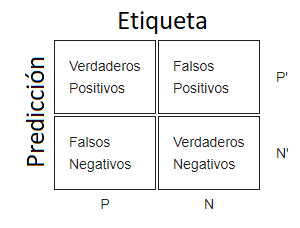
\includegraphics[width=0.5\textwidth]{../img/matrizconfusion.png}
	\caption[Disposición de la matriz de confusión.]{Disposición de la matriz de confusión~\cite{wiki:roc}.}
	\label{fig:matrizconfusion}
\end{figure}  

\subsection{Área bajo la curva ROC (\textit{AUC})}

A partir de los valores anteriores se pueden calcular los siguientes: 

\begin{itemize}
	\item \textbf{Sensibilidad o Razón de Verdaderos Positivos (TPR):}
	\begin{center}
		$TPR=\frac{TP}{P}=\frac{TP}{(TP+FN)}$ 
	\end{center} 
	\item \textbf{Razón de Falsos positivos (FPR):} 
	\begin{center}
		$FPR=\frac{FP}{P}=\frac{FP}{(FP+TN)}$ 
	\end{center} 
\end{itemize}

Algunos clasificadores binarios, como los que se usan en este trabajo, además de predecir la etiqueta de la clase a la que creen que pertenece la instancia, son capaces de devolver la probabilidad entre 0 y 1 de que la instancia pertenezca a esa clase. Usando estas probabilidades podríamos clasificar las instancias en función de un umbral, por ejemplo, una instancia sería considerada <<crisis>> si la probabilidad de que pertenezca a esa clase es mayor o igual a 0.8 y <<no crisis>> si es menor. 

El área bajo la curva ROC (\textit{Receiver Operating Characteristic}) representa la relación entre la TPR y la FPR según se varía ese umbral. Se representará la TPR en el eje $y$, y FPR en el eje $x$. Cada punto corresponderá con los valores TPR y FPR resultantes de escoger cada uno de los posibles umbrales de clasificación, y la unión de esos puntos será lo que llamamos la curva ROC del clasificador.

Nos interesa que el TPR ($sensibilidad$) sea lo mayor posible y que el FPR ($1-especificidad$) sea lo menor posible, por lo que el clasificador óptimo corresponderá con aquel que presenta un área bajo la curva ROC (AUC) igual a 1, mientras que el peor clasificador será aquel con un AUC igual a 0.5, ya que ofrecería una predicción equivalente a lanzar una moneda al aire. 

\begin{figure}[H]
	\centering
	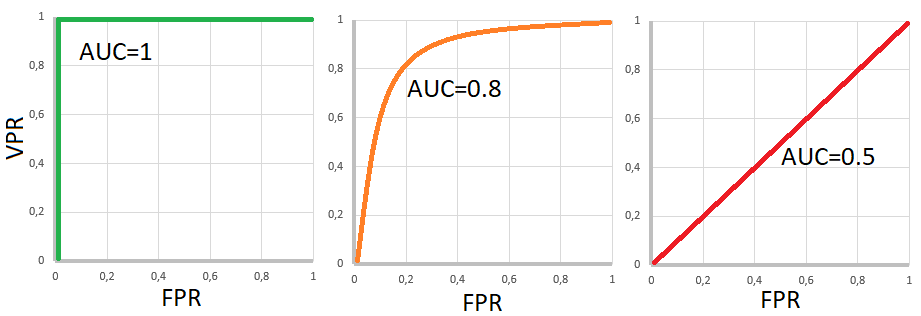
\includegraphics[width=0.7\textwidth]{../img/roc.png}
	\caption{ROC. De izquierda a derecha: mejor caso, caso intermedio y peor caso.}
	\label{fig:roc}
\end{figure} 

\subsection{Precisión media}

Se definen las siguientes variables: 
\begin{center}
	$Precision=\frac{TP}{TP+FP}$
\end{center}
\begin{center}
	$Recall=\frac{TP}{TP+FN}$
\end{center}

La precisión media (AV)~\cite{precisionrecall} se define como lo siguiente: 

\begin{center}
	$AV=\sum_{i=1}^{n}(Recall_{i}-Recall_{i-1})Precission_{i}$
\end{center}

\noindent donde $Precission_{i}$ y $Recall_{i}$ son los valores de \textit{Precision} y \textit{Recall} calculados para el umbral de clasificación i-ésimo, y \textit{n} el número de posibles umbrales. Cuanto mayor sea este valor, mejor se considera el clasificador. 

\section{Presentación del conocimiento}

En este caso una posible presentación útil del conocimiento adquirido sería la representación de la probabilidad de pertenencia a la clase <<crisis>> de cada instancia ordenadas cronológicamente, es decir, cómo varía la probabilidad de crisis epiléptica del paciente con el tiempo en función del modelo. Esta será una de las gráficas que serán visibles en la aplicación de Android desarrollada. 

\begin{figure}[H]
	\centering
	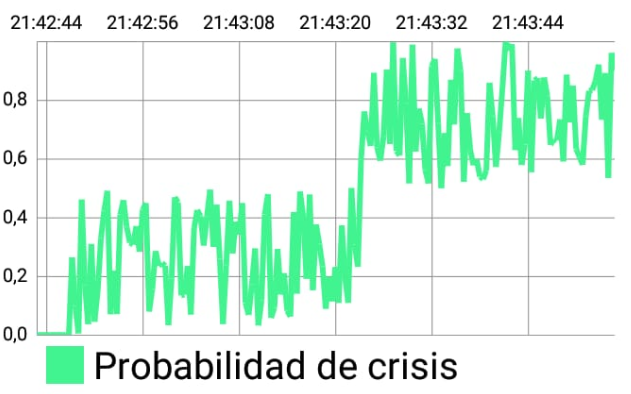
\includegraphics[width=0.7\textwidth]{../img/prob.png}
	\caption{Ejemplo de representación de la probabilidad de crisis en función del tiempo.}
	\label{fig:prob}
\end{figure} 

